\documentclass{beamer}
\usepackage{beamerthemesplit}
\usepackage{graphics}
%\usepackage[lined,boxed]{algorithm2e}
\usepackage[lined,noend]{algorithm2e}
\usepackage{amsmath}
\usepackage{tikz}
\usetikzlibrary{positioning,shapes.multipart}
\usepackage{amssymb}
\usepackage{listings}
\usepackage{soul}
\usepackage{mathtools}
\usepackage{colortbl}
\usepackage{subfigure}
\newcommand{\given}[0]{\ensuremath{\!\mid\!}}
\makeatletter
\newcolumntype{W}{!{\smash{\vrule
\@width 4\arrayrulewidth
\@height\dimexpr\ht\@arstrutbox+2pt\relax
\@depth\dimexpr\dp\@arstrutbox+2pt\relax}}}
\makeatother
\definecolor{gray}{rgb}{.7,.7,.7}



\DeclarePairedDelimiter\ceil{\lceil}{\rceil}
\DeclarePairedDelimiter\floor{\lfloor}{\rfloor}

\lstset{
basicstyle=\small,
keywordstyle=\color{blue}\bfseries,
numbers=left,
numberstyle=\tiny,
numbersep=5pt,
showstringspaces=false,
showspaces=false,
captionpos=b,
frame=tb,
float=tbh,
,escapeinside={*@}{@*}
}
\usetheme{Boadilla}
\title{ Analysis of Algorithms}
\subtitle{Coping With NP Completeness}
\author{Hikmat Farhat}
%\email{hfarhat@ndu.edu.lb}
%\institution{Notre Dame University}
\newtheorem{mydef}{Definition}
\newtheorem{lem}{Lemma}
%\newcommand{\emphasis}[1]{\textcolor{yellow}{#1}}
%\newcommand{\emphasis}[1]{\hl{#1}}
\newcommand{\emphasis}[1]{\ul{#1}}
%\newcommand{\floor}[1]{\lfloor{#1}\rfloor}
%\newcommand{\bfloor}[1]{\Big\lfloor{#1}\Big\rfloor}

%\newcommand{\gets}[0]{\leftarrow}

%\newcommand{\gets}{\ensuremath{\leftarrow}}
%\DeclareTextFontCommand{\emph}{\emphasis}
\sethlcolor{yellow}
\begin{document}
% title page
\frame{\titlepage}

\begin{frame}
  \frametitle{Coping with NP-complete problems}
  \begin{itemize}
  \item It \textbf{seems} impossible to solve NP-complete problems in polynomial time
  \item We can try to find an "efficient" non-polynomial time algorithm
  \item Basically find a solution without using brute force (i.e. trying all possibilities)
  \item Brute force for  3SAT
    \begin{itemize}
    \item Given a 3SAT instance with $n$ variables
    \item try all possible $2^n$ assignments
    \item if formula not satisfiable then we have to go through all $2^n$ possibilities
    \item Complexity $O(n^3\cdot 2^n)$. Why ?
    % there are n choose 3 ways of selecting clauses which is O(n^3)
     \item Because evaluating each clause takes constant time
    \item There are at most $n$ choose 3 clauses $\binom{n}{3}=\frac{n!}{(n-3)!3!}=O(n^3)$
    \end{itemize}
  \end{itemize}
\end{frame}
\section{Backtracking}
\begin{frame}
  \frametitle{SAT}
  \begin{itemize}
    \item Can we do better?
   \item Construct a solution, if possible, step by step
   \item If current partial  solution cannot be extended to a valid solution: backtrack
  \item Consider the formula below: if we assign the true value to variable $x$:
  \begin{enumerate}
    \item Remove all clauses containing $x$ since they are satisfied
    \item Remove $\bar{x}$ from all clauses    
  \end{enumerate}
  \item Note that an empty clause is \textbf{ unsatisfiable}
  \end{itemize}
  \begin{align*}
    (x_1\vee x_2\vee x_3\vee x_4)\wedge(\bar{x}_1)\wedge(x_1\vee x_2\vee\bar{x}_3)\wedge(x_1\vee\bar{x}_4)\wedge(x_2\vee\bar{x}_4)
  \end{align*}
\end{frame}
\begin{frame}
  \frametitle{Backtracking example}
\begin{itemize}
 \item As can be seen from the backtracking below the formula is satisfiable with 
 \item $x_1=False, x_2=True, x_4=False$ and $x_3$ can be either True or False 
\end{itemize}
\begin{tikzpicture}[thick,scale=0.8, every node/.style={transform shape}]
\node[draw] (A){$ (x_1\vee x_2\vee x_3\vee x_4)\wedge(\bar{x}_1)\wedge(x_1\vee x_2\vee\bar{x}_3)\wedge(x_1\vee\bar{x}_4)\wedge(x_2\vee\bar{x}_4)$};
\node[draw,node distance=1 and -6,below left=of A](B){$(x_2\vee x_3\vee x_4)\wedge (x_2\vee\bar{x}_3)\wedge(\bar{x}_4)\wedge (x_2\vee\bar{x}_4)$};
\draw[->](A) edge  node [above,font=\tiny] {$x_1=0$} (B);
\node[draw,node distance=1 and -4,below left=of B](C){$(x_3\vee x_4)\wedge(\bar{x}_3)\wedge(\bar{x}_4)$};
\draw[->](B) edge node[left,font=\tiny] {$x_2=0$} (C);
\node[draw,node distance=0.5, below left=of C](D){$(x_4)\wedge(\bar{x}_4)$};
\draw[->](C) edge node[below,font=\tiny] {$x_3=0$} (D);
\node[draw,node distance=0.5,below left=of D](E){$()$};
\draw[->](D) edge node[right,font=\tiny]{$x_4=0$}(E);
\node[draw,node distance=0.5,below right=of D](F){$()$};
\draw[->](D) edge node[left,font=\tiny]{$x_4=1$}(F);
\node[draw,node distance=0.5 and -1,below right=of C](G){$()\wedge (\bar{x}_4)$};
\draw[->](C) edge node[right,font=\tiny]{$x_3=1$}(G);
\node[draw,node distance=1 and -2,below right=of B](H){$(\bar{x}_4)$};
\draw[->](B) edge node[right,font=\tiny]{$x_2=1$}(H);
\node[draw,node distance=1 and -2,below right=of A](I){$()\wedge(x_2\vee\bar{x}_4)$};
\draw[->](A) edge node[above,font=\tiny]{$x_1=1$}(I);
\end{tikzpicture}
\end{frame}


\begin{frame}[fragile]
  \frametitle{Solving 3SAT using backtracking}
  \begin{itemize}
  \item Let $\phi=C_1\wedge C_2\wedge\ldots\wedge C_k$ be a 3SAT formula with $n$ variables
   and $k$ clauses.
  \item If $\phi$ is empty, i.e. has no clauses, then it is trivially satisfiable.
  \item If $\phi$ has at least one clause we can write
    \begin{align*}
      \phi&=(x\vee y\vee z)\wedge \phi'\\
          &=(x\wedge\phi')\vee (y\wedge\phi')\vee (z\wedge\phi')
    \end{align*}
  \item So we reduce the 3SAT with $n$ variables to three probems with $n-1$ variables.
  \item We obtain the recurrence
  \begin{align*}
    T(n)=3T(n-1)+O(n^3)
  \end{align*}
  \item With a solution of $T(n)=O(n^33^n)$. Which is worse than before !
  \end{itemize}
\end{frame}
\begin{frame}
  \begin{itemize}
    \item We are doing unnecessary work.
\item Now $x\wedge\phi$ is true if both terms are true which is equivalent to $\phi'\given x$
(i.e. $\phi'$ is sat given that $x$ is true)
\item If $\phi'\given x$ is not satisfiable then $y\wedge\phi'$ is satisfiable 
iff $\phi'\given\bar{x}y$
\item Finally, if both $\phi'\given x$ and $\phi'\given \bar{x}y$ are not satisfiable then 
$z\wedge\phi'$  is satisfiable iff $\phi'\given \bar{x}\bar{y}z$ is.
\item The above suggests the following algorithm for solving a 3SAT formula
  \end{itemize}
\end{frame}




\begin{frame}[fragile]

  \begin{algorithm}[H]
    \DontPrintSemicolon
    \SetKwFunction{SolveSAT}{SolveSAT}
    \SolveSAT($\phi$)\; 

    \If{$\phi=\emptyset$}{\Return True\;}
    \If{$\phi$ contains an empty clause}{\Return False\;}
    Decompose $\phi=(x\vee y\vee z)\wedge\phi'$\;
    \If{\SolveSAT($\phi\vert x$)}{\Return True\;}
    \If{\SolveSAT($\phi\vert\bar{x}y$)}{\Return True\;}
    \Return\SolveSAT($\phi\vert\bar{x}\bar{y}z$)\;
  \end{algorithm}
  \begin{itemize}
  \item The SolveSAT function obeys the recurrence
    \begin{align*}
      T(n)=T(n-1)+T(n-2)+T(n-3)+O(n^k)
    \end{align*}
\item Which has a solution (see later) $O(1.839^n)$
  \end{itemize}
\end{frame}


\section{Solving recurrences: annihilator method}
\begin{frame}
  \frametitle{Annihilator method}
  \begin{itemize}
  \item An operator takes functions as input to produce different functions.
  \item We will use the following operators
    \begin{enumerate}
    \item Sum of two functions $(f+g)(n)=f(n)+g(n)$
    \item Scale of a function $(\alpha\cdot f)(n)=\alpha\cdot f(n)$
   \item Shift (right) $(E\cdot f)(n)=f(n+1)$.
    \end{enumerate}
  \item An annihilator is an \textbf{operator}  that transforms a function into a null function.
  \item For example, let $f(n)=2^n$ then $(E-2)f(n)=(E-2)2^n=2^{n+1}-2\cdot 2^n=0$ 
  \end{itemize}
\end{frame}
\begin{frame}
  \begin{itemize}
  \item In general $(E-c)\alpha\cdot a^n=\alpha\cdot a^{n+1}-\alpha\cdot c\cdot a^n=\alpha\cdot (a-c)\cdot a^n$. This is null \textbf{iff} $c=a$.
  \item Also, if $c\neq a$ then $(E-c)a^n=constant\cdot a^n$
  \item How does that help us in solving recurrences?
  \item Consider the following recurrence
    \begin{align*}
      &T(n)=3T(n-1)\\
   \Rightarrow &T(n+1)-3T(n)=0\\
   \Rightarrow &ET(n)-3T(n)=0\\
   \rightarrow &(E-3)T(n)=0\\
   \Rightarrow & T(n)=\alpha\cdot 3^n \text{ for some constant }\alpha
 \end{align*}
  \end{itemize}
\end{frame}

\begin{frame}
  \begin{itemize}
  \item We saw from the above that for the shift operator

    \begin{align*}
      (E-c)\alpha\cdot a^n=\alpha\cdot (E-c)a^n
    \end{align*}
\item Then if we have $\alpha a^n+\beta b^n$ it follows that 
  \begin{align*}
    (E-b)(E-a)(\alpha a^n+\beta b^n)=(E-b)\gamma b^n=\gamma (E-b)b^n=0
  \end{align*}
\item In general, for \textbf{distinct} $a_0,\ldots, a_k$ 
  \begin{align*}
   (E-a_0)(E-a_1)\ldots (E-a_k)\left[\sum_{i=0}^k\alpha_ia_i^n \right]=0 
  \end{align*}
  \end{itemize}
\end{frame}
\begin{frame}
  \frametitle{Polynomials}
  
  \begin{itemize}
  \item Consider the function $\alpha\cdot n+\beta$
  \item $(E-1)\alpha n=\alpha(n+1)+\beta-\alpha n-\beta=\alpha$
  \item So $(E-1)^2(\alpha n+\beta)=0$
  \item In general if $(E-1)^kF(n)=0$ then
    \begin{align*}
      F(n)=\sum_{i=0}^{k-1}\alpha_in^i
    \end{align*}
\item Also $(E-a)^kF(n)=0$ then
  \begin{align*}
    F(n)=\left(\sum_{i=0}^{k-1}\alpha_in^i\right)\cdot a^n 
  \end{align*}
  \end{itemize}
\end{frame}
\begin{frame}
  \frametitle{Fibonacci}
  \begin{itemize}
  \item Recall that the Fibonacci sequence obeys the following recurrence
    \begin{align*}
      &F(n+2)=F(n+1)+F(n)\\
    \Rightarrow & E^2F(n)-EF(n)-F(n)=0\\
    \Rightarrow & (E^2-E-1)F(n)=0\\
    \end{align*}
\item The above can be factored as 
  \begin{align*}
    (E-\phi)(E-\hat{\phi})F(n)=0
  \end{align*}
\item Where $\phi=\frac{1+\sqrt{5}}{2}$ and $\hat{\phi}=1-\phi$.
\item Therefore
  \begin{align*}
    F(n)=\alpha \phi^n+\beta \hat{\phi}^n
  \end{align*}
  \end{itemize}
\end{frame}
\begin{frame}
  \begin{itemize}
  \item The values of $\alpha$ and $\beta$ are determined from the boundary conditions
$F(0)=0$ and $F(1)=1$ thus $\alpha=-\beta=\frac{1}{\sqrt{5}}$ and we get
\begin{align*}
  F(n)=\frac{1}{\sqrt{5}}\phi^n-\frac{1}{\sqrt{5}}(1-\phi)^n
\end{align*}

  \end{itemize}
\end{frame}
\begin{frame}
  \frametitle{Tower of Hanoi}
\begin{itemize}
  \item Remember for the Tower of Hanoi the recurrence was
  \begin{align*}
    T(n)=2T(n-1)+1
  \end{align*}
  \item using $E$
  \begin{align*}
    (E-2)T-1=0
  \end{align*}
  \item This is the first time we see a non homogeneous 
\end{itemize}
  

\end{frame}
\begin{frame}
  \frametitle{AVL Tree}
  \begin{itemize}
  \item Recall an AVL tree has the property that the left and right subtrees cannot have a height difference more than 1.
\item Consider the \textbf{smallest} (in terms of number of nodes) AVL tree of height $h$.
\item Since the tree is the smallest then the left tree has height $h-1$ and the right has height $h-2$ (or vice versa).
\item Therefore the smallest AVL of height $h$ obeys the recurrence
  \begin{align*}
   &N(h)=N(h-1)+N(h-2)+1 \\
\Rightarrow N(h+2)-N(h+1)-N(h)=1\\
\Rightarrow (E^2-E-1)N(h)=1
  \end{align*}
\item The solution is
  \begin{align*}
    N(h)=\alpha \phi^h+\beta \hat{\phi}^h+\gamma
  \end{align*}
  \end{itemize}
\end{frame}
\begin{frame}
  \begin{itemize}
  \item We can determine the constants $\alpha,\beta,\gamma$ by using the boundary conditions $ N(0)=1, N(1)=2 ,N(2)=4$

\item We need the asymptotic behavior, for large $h$
  \begin{align*}
    N(h)=\Omega( \phi^h)
  \end{align*}
\item Therefore 
  \begin{align*}
    h=O(\log n)
  \end{align*}
  \end{itemize}
\end{frame}


% \begin{frame}
%   \frametitle{n Queens}
%    \begin{algorithm}[H]

%    \DontPrintSemicolon
%   \SetKwFunction{RNQueens}{RNQueens}

% \RNQueens(Q,r) 
%  \BlankLine
% \If{$r=n+1$}{
%   Print Q\;
% }
% \Else{
% %\nl \For{$i=1$ \KwTo $n$}{
% \For{$i=1$ \KwTo $n$}{
%   Try all columns\;
%      $legal\gets True$\;
%      \For{$j=1$ \KwTo $r-1$}{
%        check all previous rows\;
%       \If{$Q[j]=i$ or $(Q[j]=i+r-j)$ or $(Q[j]=i-r+j)$}
%       {
%         $legal\gets False$\;
%       }
%      }
%      \If{$legal$}{
%       $Q[r]\gets i$\;
%       \RNQueens(Q,r+1)\;
%      }
% }
% }
% \end{algorithm}
% \end{frame}


\section{Branch and Bound}

\subsection{Knapsack}


\begin{frame}
  \frametitle{Branch and Bound: Knapsack}
  \begin{itemize}
  \item We compute an upper bound using the greedy solution for the fractional knapsack

  \begin{align*}
    S=v_1+v_2+\ldots +v_k+\frac{W-w_1-\ldots -w_k}{w_{k+1}}v_{k+1}
  \end{align*}
\item But since
  \begin{align*}
    \frac{v_1}{w_1}> \frac{v_2}{w_2}>\ldots >\frac{v_k}{w_k}
  \end{align*}

\item Then we can write
  \begin{align*}
    S&\le \frac{w_1}{w_1}v_1+\frac{w_2}{w_1}v_1+\ldots +\frac{w_k}{w_1}v_1+\frac{W-w_1-\ldots -w_k}{w_{1}}v_{1}\\
    S&\le W\cdot \frac{v_1}{w_1}
  \end{align*}

  \end{itemize}
\end{frame}
\begin{frame}
  \begin{itemize}
  \item Assuming that items are sorted by descending $\frac{v}{w}$ we use backtracking with the same order of selection for the items
  \item At each step, given a knapsack of size $W$ and a list of unused items 
  \item We have an upper bound for the entire branch
  \item As an example assume we have a knapsack of capacity $W=11$ and the following items
  \end{itemize}
  \begin{tabular}[h]{c|c|c|}
   item & Value & Weight\\
\hline
   1 & 1 &1\\
   2 & 2 & 3\\
   3 & 3 & 5\\
   4 & 4 & 7
  \end{tabular}
\end{frame}
\begin{frame}
\def\textA{{\scriptsize $v=0,w=0$}
\nodepart{two}
{\scriptsize $ub=11\times 1=11$}
}

\def\textB{{\scriptsize $v=1,w=1$}
\nodepart{two}
{\scriptsize $ub=1+10\times 0.66=7.6$}
}

\def\textC{{\scriptsize $v=3,w=4$}
\nodepart{two}
{\scriptsize $ub=3+7\times 0.6=7.2$}
}

\def\textD{{\scriptsize $v=1,w=1$}
\nodepart{two}
{\scriptsize $ub=1+10\times 0.6=7$}}

\def\textE{{\scriptsize $v=6,w=9$}
\nodepart{two}
{\scriptsize $v=6$(items 1,2,3)}}

\def\textF{{\scriptsize $v=3,w=4$}
\nodepart{two}
{\scriptsize $ub=7$}

}

%\def\textF{$\text{min}\  x_1-2x_2$
%\nodepart{two}
%{\scriptsize $x_1^*=1,x_2^*=2.1667$}}

\def\textG{{\scriptsize $v=2,w=3$}
\nodepart{two}
{\scriptsize $ub=2+8\times 0.6=6.8$}

}

\def\textH{{\scriptsize $v=7,w=11$}
\nodepart{two}
{\scriptsize $v=7(items 1,2,4)$}}

% \begin{frame}
%   \begin{tikzpicture}[thick,scale=0.6, every node/.style={transform shape}]
% %% node type: when drawn its a rectangle
% %% split and split parts: determine how many parts it has
% %#% draw: means draw the boundary otherwise no boundary is drawn
%    \node[rectangle split, rectangle split parts=3,draw] (A){"A" \nodepart{two} "B"};
%   \end{tikzpicture}
% \end{frame}


\tikzset{>=stealth,parent node/.style={rectangle split, rectangle split parts=2,align=left,text width=3cm,draw,node distance=1cm and 1cm}}


\begin{figure}
\centering

\begin{tikzpicture}[thick,scale=0.6, every node/.style={transform shape}]
\node[parent node ](A){\textA};
\node[parent node,node distance =1 and 0.3,below right =of A](K){{\scriptsize $v=0,w=0$}\nodepart{two} {\scriptsize $ub=11\times 0.66=7.26$}};
\node[parent node,node distance =1 and 3.3,below left =of A](B){\textB};
\node[parent node,node distance =1 and 0.3,below left =of B](C){\textC};
\node[parent node,node distance =1 and -0.3, below right =of B](D){\textD};
\node[parent node,node distance=1 and 0.3,below left =of C](E){\textE};
\node[parent node,node distance=1 and 0.3,below right =of C](F){\textF};
\node[parent node,node distance=1 and 0.3,below left =of K](G){\textG};
\node[parent node,node distance=1 and 0.3,below left=of F](H){\textH};
\node[parent node,node distance=2 and 0, below =of K](I){{\scriptsize $v=0,w=0$} \nodepart{two}{\scriptsize $ub=11\times 0.6=6.6$}};
\node[parent node,node distance=1 and 0.3,below right=of F](J){{\scriptsize $v=3,w=4$}\nodepart{two} {\scriptsize $v=3(items 1,2)$}};

\draw[->](A.south)--(0,-1.)-|(B)node[above, near start]{\scriptsize $w 1$} node[left,near end]{\scriptsize $1$};
\draw[->](A.south)-+(0,-1)-|(K) node[above,near start]{\scriptsize $w/1$} node[right, near end]{{\scriptsize 2}};

\draw[->](B.south) -- +(0,-0.5)-|(C) node[above,near start]{\scriptsize $w 2$} node[left,near end]{\scriptsize $3$};
\draw[->](B.south) -- +(0,-0.5)-|(D)node[above,near start]{\scriptsize $w/2$} node[right,near end]{\scriptsize $4$};
\draw[->](C.south) -- +(0,-0.5)-|(E)node[above,near start]{\scriptsize $w 3$}node[left,near end]{\scriptsize $5$};

\draw[->](C.south) -- +(0,-0.5) -| (F) node[above,near start]{\scriptsize $w/3$}node[right,near end]{\scriptsize $6$};
\draw[->](F.south) -- +(0,-0.5) -| (H) node[above,near start]{\scriptsize $w 4$}node[left, near end]{\scriptsize $7$};

\draw[->](F.south) -- +(0,-0.5) -|(J) node[above,near start]{\scriptsize $w/4$}node[right,near end]{\scriptsize $8$};
\draw[->](K.south) -- +(0,-0.5) -|(G) node[above,near start]{\scriptsize $w 2$}node[left,midway]{\scriptsize $9$};
\draw[->](K.south) -- +(0,-0.5) -|(I) node[right,near start]{\scriptsize $w/2$}node[right,near end]{\scriptsize $10$};
\end{tikzpicture}
\caption{Branch and Bound for Knapsack instance}
\end{figure}

\end{frame}

\begin{frame}
  \frametitle{Example2}
  \begin{itemize}
  \item Consider the following instance with the knapsack weight $W=7$
  \end{itemize}
   \begin{tabular}[h]{c|c|c|c|}
   item & Value & Weight & density\\
\hline
   1 & 8 &5 &1.6\\
   2 & 6 & 4 & 1.5\\
   3 & 2 & 2 & 1\\
   4 & 1 & 1 & 1
  \end{tabular}
\end{frame}


\begin{frame}
\def\textA{{\scriptsize $v=0,w=7$}
\nodepart{two}
{\scriptsize $ub=7\times 1.6=11.2$}
}

\def\textB{{\scriptsize $v=8,w=2$}
\nodepart{two}
{\scriptsize $ub=8+2\times 1.5=11$}
}

\def\textC{{\scriptsize $w_2=4>2$}
\nodepart{two}
{\scriptsize Not feasible}
}

\def\textD{{\scriptsize $v=8,w=2$}
\nodepart{two}
{\scriptsize $ub=8+2\times 1=10$}}

\def\textE{{\scriptsize $v=6,w=9$}
\nodepart{two}
{\scriptsize $v=6$(items 1,2,3)}}

\def\textF{{\scriptsize $v=10,w=0$}
\nodepart{two}
{\scriptsize items(1,3)}

}

%\def\textF{$\text{min}\  x_1-2x_2$
%\nodepart{two}
%{\scriptsize $x_1^*=1,x_2^*=2.1667$}}

\def\textG{{\scriptsize $v=6,w=2$}
\nodepart{two}
{\scriptsize $ub=6+2\times 1=8$}

}

\def\textH{{\scriptsize $v=7,w=11$}
\nodepart{two}
{\scriptsize $v=7(items 1,2,4)$}}

% \begin{frame}
%   \begin{tikzpicture}[thick,scale=0.6, every node/.style={transform shape}]
% %% node type: when drawn its a rectangle
% %% split and split parts: determine how many parts it has
% %#% draw: means draw the boundary otherwise no boundary is drawn
%    \node[rectangle split, rectangle split parts=3,draw] (A){"A" \nodepart{two} "B"};
%   \end{tikzpicture}
% \end{frame}


\tikzset{>=stealth,parent node/.style={rectangle split, rectangle split parts=2,align=left,text width=3cm,draw,node distance=1cm and 1cm}}


\begin{figure}
\centering

\begin{tikzpicture}[thick,scale=0.6, every node/.style={transform shape}]
\node[parent node ](A){\textA};
\node[parent node,node distance =1 and 0.3,below right =of A](K){{\scriptsize $v=0,w=7$}\nodepart{two} {\scriptsize $ub=7\times 1.5=10.5$}};
\node[parent node,node distance =1 and 3.3,below left =of A](B){\textB};
\node[parent node,node distance =1 and 0.3,below left =of B](C){\textC};
\node[parent node,node distance =1 and -0.3, below right =of B](D){\textD};
%\node[parent node,node distance=1 and 0.3,below left =of C](E){\textE};
\node[parent node,node distance=1 and 0.3,below right =of C](F){\textF};
\node[parent node,node distance=1 and 0.3,below left =of K](G){\textG};
%\node[parent node,node distance=1 and 0.3,below left=of F](H){\textH};
\node[parent node,node distance=2 and 0, below =of K](I){{\scriptsize $v=0,w=7$} \nodepart{two}{\scriptsize $ub=7\times 1=7$}};
%\node[parent node,node distance=1 and 0.3,below right=of F](J){{\scriptsize $v=3,w=4$}\nodepart{two} {\scriptsize $v=3(items 1,2)$}};

\draw[->](A.south)--(0,-1.)-|(B)node[above, near start]{\scriptsize $w 1$} node[left,near end]{\scriptsize $1$};
\draw[->](A.south)-+(0,-1)-|(K) node[above,near start]{\scriptsize $w/1$} node[right, near end]{{\scriptsize 2}};

\draw[->](B.south) -- +(0,-0.5)-|(C) node[above,near start]{\scriptsize $w 2$} node[left,near end]{\scriptsize $3$};
\draw[->](B.south) -- +(0,-0.5)-|(D)node[above,near start]{\scriptsize $w/2$} node[right,near end]{\scriptsize $4$};
%\draw[->](C.south) -- +(0,-0.5)-|(E)node[above,near start]{\scriptsize $w 3$}node[left,near end]{\scriptsize $5$};

\draw[->](D.south) -- +(0,-0.5) -| (F) node[above,near start]{\scriptsize $w3$}node[right,near end]{\scriptsize $6$};
%\draw[->](F.south) -- +(0,-0.5) -| (H) node[above,near start]{\scriptsize $w 4$}node[left, near end]{\scriptsize $7$};

%\draw[->](F.south) -- +(0,-0.5) -|(J) node[above,near start]{\scriptsize $w/4$}node[right,near end]{\scriptsize $8$};
\draw[->](K.south) -- +(0,-0.5) -|(G) node[above,near start]{\scriptsize $w 2$}node[left,midway]{\scriptsize $9$};
\draw[->](K.south) -- +(0,-0.5) -|(I) node[right,near start]{\scriptsize $w/2$}node[right,near end]{\scriptsize $10$};
\end{tikzpicture}
\caption{Branch and Bound for Knapsack instance}
\end{figure}

\end{frame}

\subsection{Subset sum}
\begin{frame}
  \frametitle{Subset Sum}
\begin{itemize}
  \item At each step keep two variables: $sum$ and $remainder$
  \item The $sum$ denotes the current sum and the $remainder$ denotes the sum of all items that have not been used yet.
  \item Let $t$ be the target. Given a choice between adding/not adding element with value $v$
  \begin{enumerate}
    \item if $sum+v=t$ then solution found, return solution.
    \item if $sum+v>t$ backtrack, do not include $v$
    \item if $sum+remainder-v<t$ backtrack .
  \end{enumerate}
\end{itemize}
  

\end{frame}
\subsection{Clique}


\begin{frame}
  \frametitle{Clique}
  \begin{itemize}
  \item Recall that given a graph $G=\langle V,E\rangle$ a subset $S\subseteq V$ is said to be a \textbf{clique} iff for all $u,v\in S$ then $(u,v)\in E$.
\item We also saw that if $G$ has a \textbf{clique} of size $k$ then $\bar{G}=\langle V,\bar{E}\rangle$ has an \textbf{independent se}t of size $k$, where $(u,v)\in E$ iff $(u,v)\notin E$
\item We will use branch and bound to find a clique of maximum size in a given graph
\item First we develop  lower and upper bounds for the clique problem.
  \end{itemize}
\end{frame}
\begin{frame}
  \frametitle{Upper bound: greedy k-coloring}
  \begin{itemize}
  \item Given a graph $G=\langle V,E\rangle$ we need to color it using $k$-colors.
  \item First assign a number to each color: $1,2,\ldots,k$.
  \item Choose a vertex $v$ and assign to it the \textbf{lowest} number that is not used by its neighbors.
  \end{itemize}
\end{frame}
\begin{frame}
   \frametitle{Example}
  \begin{itemize}
  \item We use the greedy coloring to the graph shown below were nodes are considered in alphabetical order.
  \item The colors are numbered as $\{Red=1,Green=2,Blue=3,Yellow=4,Magenta=5,\ldots\}$
  \end{itemize}
  \begin{center}
    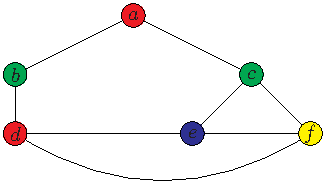
\includegraphics{coping-figs/greedy-kcolor-not-always}
  \end{center}
\end{frame}
\begin{frame}
  \frametitle{Greedy coloring not optimal, used as upper bound}
  \begin{itemize}
  \item The greedy coloring in the previous example used 4 colors
  \item An optimal coloring, as shown below, uses only 3 colors
  \end{itemize}
  \begin{center}
    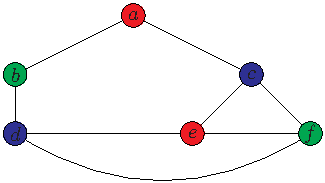
\includegraphics{coping-figs/not-greedy-less}
  \end{center}
  \begin{itemize}
  \item But greedy coloring gives an \textbf{upper bound}:
  \item For any graph optimal coloring $\le $ greedy coloring
  \end{itemize}
\end{frame}
\begin{frame}
  \frametitle{How is that used for Clique?}
  \begin{itemize}
  \item Suppose a graph $G=\langle V,E\rangle$ has a \textbf{Clique of size} $k$.
  \item Then $G$ \textbf{cannot be colored by less} than $k$ colors
  \item \textbf{Conversely}, if a graph has a $k$ coloring then
  \item \textbf{The size of maximal Clique} $\le k$.
  \item Let $k_g$ be the number of colors obtained by greedy coloring
  \item Since $k_g$ is an upper bound for coloring
  \item \textbf{Then the size of maximal Clique} $\le k_g$
  \end{itemize}
\end{frame}
\begin{frame}
  \frametitle{Lower Bound: greedy Clique}
  \begin{itemize}
  \item Given a graph $G=\langle V,E\rangle$ we can obtain a Clique using a greedy strategy as follows
    \begin{enumerate}
    \item $C\leftarrow\emptyset$
    \item Select the highest degree vertex $v$ from $V-C$ and added to $C$
    \item Remove all nodes that are not connected to $v$ from $V$
    \item repeat until $V$ is empty
    \end{enumerate}
  \end{itemize}
\end{frame}


\begin{frame}
  \frametitle{Greedy Clique Example}
  \begin{figure}[h]
    \centering
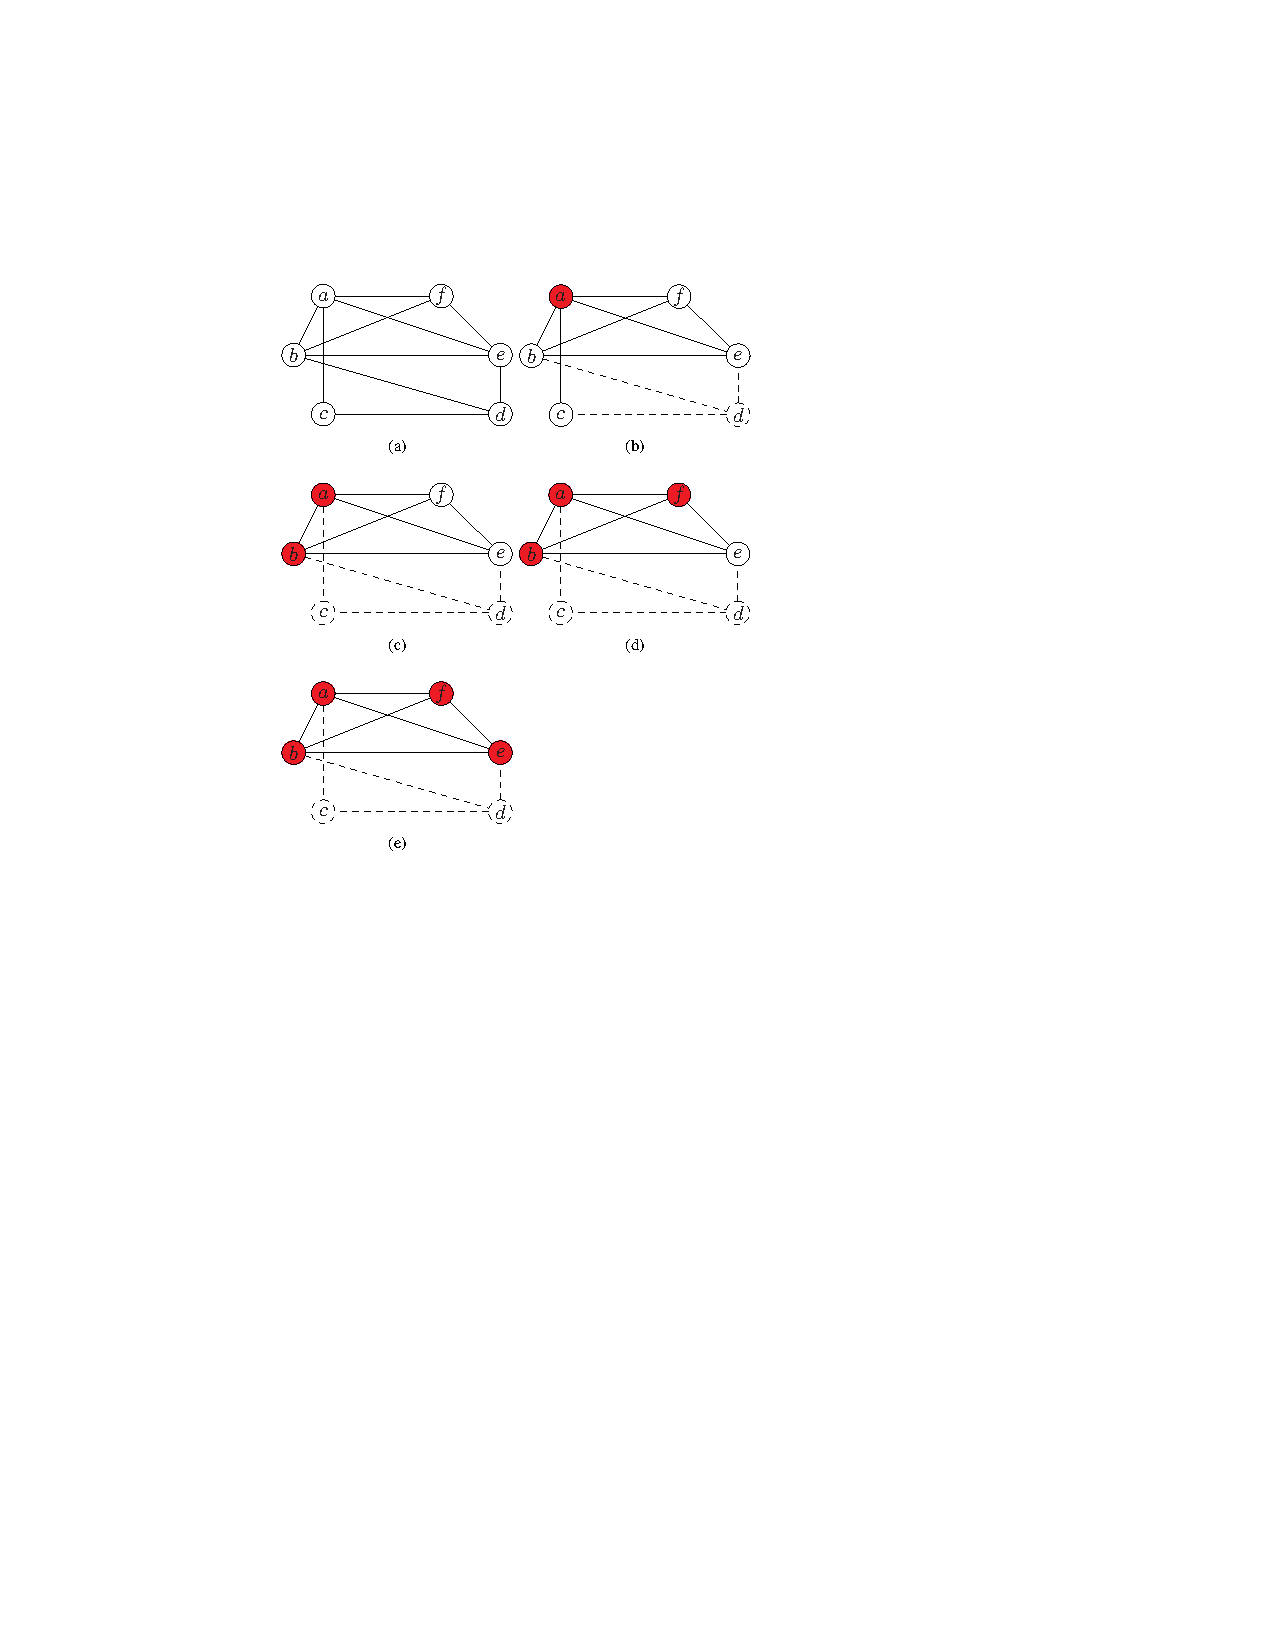
\includegraphics[width=0.5\textwidth]{coping-figs/greedy-clique}
  \end{figure}
\end{frame}

% \begin{frame}
%   \frametitle{Does it always give optimal result?}
  
% \end{frame}
\begin{frame}
  \frametitle{Clique Branch-and-Bound}
  \begin{itemize}
  \item As an example for using branch-and-bound for clique using the already discussed upper and lower bounds
  \item See the paper by Dawn M. Strickland on blackboard.
  \end{itemize}
\end{frame}
% \begin{frame}
% \tikzset{>=stealth,parent node/.style={rectangle split, rectangle split parts=2,align=left,text width=3cm,draw,node distance=1cm and 1cm}}
%   \begin{tikzpicture}[thick,scale=0.6, every node/.style={transform shape}]
%     \node[parent node](1){{\scriptsize start}\nodepart{two} {\scriptsize $lb=3+4+2+4=13$}};
%     \node[parent node,node distance=1 and 4,below left =of 1](2){{\scriptsize $a\leftarrow 1$}\nodepart{two} {\scriptsize $lb=6+4+2+4=16$}};
%     \node[parent node,node distance=1 and .1,below left =of 1](3){{\scriptsize $a\leftarrow 2$}\nodepart{two} {\scriptsize $lb=3+5+2+4=14$}};
%     \node[parent node,node distance=1 and .1,below right =of 1](4){{\scriptsize $a\leftarrow 3$}\nodepart{two} {\scriptsize $lb=7+4+5+4=20$}};
%     \node[parent node,node distance=1 and 4,below right =of 1](5){{\scriptsize $a\leftarrow 4$}\nodepart{two} {\scriptsize $lb=8+4+2+6=20$}};

%     \node[parent node,node distance=1 and 2,below left=of 3](6){{\scriptsize $a\leftarrow 2,b\leftarrow 1$}\nodepart{two} {\scriptsize $lb=3+6+2+4=15$}};
%     \node[parent node,node distance=1 and 4,below =of 3](7){{\scriptsize $a\leftarrow 2,b\leftarrow 3$}\nodepart{two} {\scriptsize $lb=3+5+5+4=17$}};
%     \node[parent node,node distance=1 and 4,below right=of 3](8){{\scriptsize $a\leftarrow 2,b\leftarrow 4$}\nodepart{two} {\scriptsize $lb=3+7+2+7=19$}};

%     \node[parent node, text width=4cm,node distance=2 and 2,below =of 6](9){{\scriptsize $a\leftarrow 2,b\leftarrow 1,c\leftarrow 3,d\leftarrow 4$}\nodepart{two} {\scriptsize $v=3+6+2+4=15(optimal)$}};
%     \node[parent node,text width=4cm,node distance=2 and 2,below right=of 6](10){{\scriptsize $a\leftarrow 2,b\leftarrow 1,c\leftarrow 4 ,d\leftarrow 3$}\nodepart{two} {\scriptsize $v=3+6+8+9=26$}};
%     \draw[->](1.south)-- +(0,-0.5) -|(2)node[left,near end]{\scriptsize 1};
%     \draw[->](1.south)-- +(0,-0.5) -|(3)node[left,near end]{\scriptsize 2};
%     \draw[->](1.south)-- +(0,-0.5) -|(4)node[left,near end]{\scriptsize 3};
%     \draw[->](1.south)-- +(0,-0.5) -|(5)node[left,near end]{\scriptsize 4};

%    \draw[->](3.south)-- +(0,-0.5) -|(6)node[left,near end]{\scriptsize 5};
%    \draw[->](3.south)-- +(0,-0.5) -|(7)node[left,near end]{\scriptsize 6};
%    \draw[->](3.south)-- +(0,-0.5) -|(8)node[left,near end]{\scriptsize 7};

%    \draw[->](6.south)-- +(0,-0.5) -|(9)node[left,near end]{\scriptsize 8};
%    \draw[->](6.south)-- +(0,-0.5) -|(10)node[left,near end]{\scriptsize 9};
%   \end{tikzpicture}
% \end{frame}

% \section{Subset Sum}
% \begin{frame}
%   \frametitle{Subset Sum}
%   \begin{itemize}
%   \item Recall that given $n$ numbers $X=\{x_1,x_2,\ldots,x_n\}$ the decision problem subset sum is given a value $t$ is there a subset  $S\subseteq X$ such that the sum of elements of $S$ is equal to $t$
% \item The corresponding optimization problem is to find the maximum sum of a subset such that the sum is less or equal to $t$
% \item For example if $X=\{1,5,2,7,16\}$ and $t=27$ then the largest sum is the sum of $\{1,2,7,16\}=26$
% \item Before we give an approximation to the problem we will give an exact algorithm.
% \item Obviously one can enumerate all subsets, take the sum of each and then find the maximum.
% \item Instead we present an exact algorithm, while still exponential in complexity, it will help us find an approximate solution 
%   \end{itemize}
% \end{frame}

% \begin{frame}
%   \begin{itemize}
%   \item The basic idea comes from the fact that subsets can be generated from smaller subsets.
%   \item Let $X=\{x_1,x_2,\ldots,x_n \}$ and $2^i$ be the set of subsets of $\{x_1,x_2,\ldots ,x_i\}$.
%   \item It is easy to verify that $2^{i+1}=2^i\cup C$ where $C=\{A\cup\{x_i\} | A\in 2^i\}$
%   \item Example: consider the set  $X=\{1,5,2,7,16\}$
%  \item $2^0=\emptyset$,
%   \item $2^1=\{\emptyset,\{1\}\}$
%   \item $2^2=\{\emptyset,\{1\},\{2\},\{1,2\}\}=\{\emptyset,1\}\cup\{\emptyset\cup\{2\},\{1\}\cup\{2\}\}$
%   \item $2^3=\{\emptyset,\{1\},\{2\},\{3\},\{1,2\},\{1,3\},\{2,3\},\{1,2,3\}\}=$
%   \end{itemize}
%   \begin{align*}
%   \{\emptyset,\{1\},\{2\},\{1,2\}\}\cup\{\emptyset\cup\{3\},\{1\}\cup\{3\},\{2\}\cup\{3\},\{1,2\}\cup\{3\}\}
%   \end{align*}
% \end{frame}

% \begin{frame}
%   \begin{itemize}
%   \item Using the relationship between subsets let $L_i$ be the set of the sums of subsets of $x_1,\ldots,x_i$ we can write
%     \begin{align*}
%       L_i=L_{i-1}\cup L_{i-1}+x_i
%     \end{align*}
%   \item Where $L_{i-1}+x_i$ is the list obtained by adding $x_i$ to every element in $L_{i-1}$
%  \item This "merging" of the sums can be done similar to the merge procedure in mergesort where duplicate entries are removed.
%  \item Given such merge procedure we can find the maximum sum less that $t$ using the following algorithm
%   \begin{algorithm}[H]

%    \DontPrintSemicolon
%   \SetKwFunction{SubsetSum}{SubsetSum}
%   \SetKwFunction{Merge}{Merge}
% \SubsetSum(X,t) 
%  \BlankLine
% \nl $n\gets|X|$\;
% \nl $L_0\gets \{0\}$\;
% \nl \For{$i=1$ \KwTo $n$}{
% \nl  $L_i=$\Merge($L_{i-1},L_{i-1}+x_i$)\;
% \nl  remove from $L_i$ all elements greater than $t$\;
% }
% \Return the largest element in $L_n$\;
% \end{algorithm}

%   \end{itemize}
% \end{frame}
% \begin{frame}
%   \frametitle{Example}
%   \begin{itemize}
%   \item We will apply the algorithm to the set $X=\{4,5,19,7,16\}$ and $t=29$ then the largest sum is the sum of% $\{1,2,7,16\}$
%   \item Iteration 1: $L_1=\{0\}\cup\{0\}+4=\{0,4\}$
% \item Iteration 2: $L_2=\{0,4\}\cup\{0,4\}+5=\{0,4,5,9\}$
% \item Iteration 3: $L_3=\{0,4,5,9\}\cup\{0,4,5,9\}+19=\{0,4,5,9,19,23,24,28\}$
% \item Iteration 4: $L_4=\{0,4,5,9,19,23,24,28\}\cup\{0,4,5,9,19,23,24,28\}+7=\{0,4,5,7,9,11,12,16,19,23,24,26,28\}$ (values $\ge 29$ were removed) 
% \item Iteration 5: $L_5=\{0,4,5,7,9,11,12,16,19,23,24,26,28\}\cup \{0,4,5,7,9,11,12,16,19,23,24,26,28\}+16 $
% $=\{0,4,5,7,9,11,12,16,19,20,21,23,24,25,26,27,28\}$ (duplicates and values $\ge 29$ were removed) 
  
%   \end{itemize}
% \end{frame}
% \section{Approximation}
% \begin{frame}
%   \frametitle{Approximation Algorithm}
%   \begin{itemize}
%   \item The approximation algorithm discuss here is based on a \textit{trimming}  procedure.
%   \item Instead of keeping all the sums, we represent all the sums that are \textit{close enough} to each other by a single value.
%   \item For example suppose that we keep a single sum for each group of sums that are within 10\% of each other. The value 10\% is a variable that
% controls how "good" we need the approximation to be. Let us call it $\delta$.
%   \item Let $L=\{10,11,12,15,20,21,22,23,24,29\}$. In this case $11\le (10+0.1\times 10)$ so we keep 10 to represent 10 and 11
%  \item similarly $21\le (20+0.1\times 20)$ and $22\le (20+0.1\times 20)$ so we keep 20 to represent 20,21 and 22. 
%  \item Finally the \textit{trimmed} list becomes $L'=\{10,12,15,20,23,29\}$
%  \item The question is: how much is the size of $L$ is \textit{reduced} by this \textit{trimming}  procedure?
%   \end{itemize}
% \end{frame}
% \begin{frame}
%   \frametitle{List size reduction}
%   \begin{itemize}
%   \item each of the sums starts with a 0 followed by some integer $z\ge 1$. The trimming procedure produces a list such that successive elements are at least $1+\delta$ apart. Let $z$ be the first non-zero element of a trimmed list $L$ and let $k$ be the number of elements in $L$ after $z$. Since successive elements of $L$ are at least $1+\delta$ apart  $L$ cannot have more elements than the list $L'$ below:
%  \item $L'=\{0,z,(1+\delta)z,(1+\delta)^2z,\ldots,(1+\delta)^kz\}$.
% \item Thus $(1+\delta)^k z\le t$ and it follows that $(1+\delta)^k\le t$ (because $z\ge 1$)
%  \item Now
%    \begin{align*}
%      k &\le \log_{1+\delta}t= \frac{\ln t}{\ln 1+\delta} &\\
%        &\le \frac{(1+\delta)}{\delta}\ln t & (\frac{x}{1+x}\le\ln x\le x)\\
%        &\le \frac{\ln t}{\delta} &
%    \end{align*}
  
%   \end{itemize}
% \end{frame}

%  \begin{frame}
%    \frametitle{Accuracy of the approximation result}
%    \begin{itemize}
%    \item As things stand we can show that the accuracy of the approximation result is $1+2n\delta$.
%    \item This means that if $y$ and $z$ are the exact and approximation results respectively then $z\le y\le (1+2n\delta)z $
%   \item We don't want the accuracy of our algorithm to depend on $n$. Let $\delta=\frac{\epsilon}{2 n}$ then $z\le y\le (1+\epsilon)\le z$
%    \item In this case the size of  $L'$ becomes $k\le \frac{2 n\ln t}{\epsilon}$.
%    \item Since our approximation algorithm is polynomial in the size of $L'$ then it is polynomial in $n$ and $\ln t$ which is the number of bits needed to represent $t$.
%    \end{itemize}
%  \end{frame}
%  \begin{frame}
%    \begin{itemize}
%    \item Consider an iteration $i$. Let $y\in P_i$ then $\exists z\in L_i$ such that $\frac{y}{(1+\delta)^i}\le z\le y$
%   \item \textbf{Proof}.
%   \item We will prove the above property by induction over $i$.
%   \item Base case.$P_1=\{0,x_1\}$ and $L_1=\{0,x_1\}$ so clearly $\frac{x_1}{(1+\delta)}\le x_1\le x_1$.
%   \item Hypothesis. Assume that for every $y\in P_i$, there exists $z\in L_i$ such that $\frac{y}{(1+\delta)}\le z\le y$.
%   \item Induction step. Consider $y\in P_{i+1}$. We have two cases $y\in P_i$ or $y=y'+x_{i+1}$ for some $y'\in P_i$
%   \item Case 1: $y\in P_i$. By hypothesis $\exists z'\in L_i$ such that $\frac{y}{(1+\delta)^i}\le z'\le y$.
%    \item Since $L_{i+1}=TRIM(MERGE(L_i,L_i+x_{i+1}))$  then either $z'\in L_i$ or $z'$ was trimmed which means that $\exists z\in L_{i+1}$ such that $z\le z'\le (1+\delta)z$
%   \item Therefore $\frac{y}{(1+\delta)^{i+1}}\le z\le y$ for some $z\in L_{i+1}$

%    \end{itemize}
%  \end{frame}

%  \begin{frame}
%    \begin{itemize}
%    \item Case 2: $y=y'+x_{i+1}$ for some $y'\in P_i$. 
%    \item We have  $L_{i+1}=TRIM(MERGE(L_i,L_i+x_{i+1}))$. Since $z'\in L_i$ then either $z'+x_{i+1}\in L_{i+1}$ or it was trimmed.
%    \item If $z'+x_{i+1}\in L_{i+1}$ then by the induction hypothesis we have
%      \begin{align*}
%        \frac{y'}{(1+\delta)^i}+x_{i+1} & \le z'+x_{i+1} \le y'+x_{i+1}=y\\
%    \frac{y'+x_{i+1}}{(1+\delta)^i} & \le z'+x_{i+1} \le y'+x_{i+1}=y
%      \end{align*}
%  \item If $z'+x_{i+1}$ was trimmed then $\exists z\in L_{i+1}$ such that $\frac{y'}{(1+\delta)}\le z\le y'$. Combining both facts we get
%    \begin{align*}
%      \frac{y'+x_{i+1}}{(1+\delta)^{i+1}} & \le z \le y'+x_{i+1}=y
%    \end{align*}
%    \end{itemize}
%  \end{frame}

% \section{Vertex Cover}

% \begin{frame}
%   \frametitle{Vertex Cover}
%   \begin{itemize}
%   \item We give an approximation algorithm that returns  a vertex cover $S\subseteq V$ of graph $G=(V,E)$. The returned VC is not the smallest one however.
%   \item The algorithm is simple. Remove an edge $(u,v)$ from $E$, add $u$ and $v$ to $S$ then remove all the edges incident on  $u$ and $v$.
%   \end{itemize}
%   \begin{algorithm}[H]

%    \DontPrintSemicolon
%   \SetKwFunction{ApproxVC}{ApproxVC}
% \ApproxVC(G) 
%  \BlankLine
% \nl $C\gets\emptyset$\;
% \nl $F\gets E$\;
% \nl \While{$F\ne\emptyset$}{
% \nl  select arbitrary edge $(u,v)$ from $F$\;
% \nl  $C\gets C\cup\{u,v\}$\;
% \nl  remove from $F$ every incident on $u$ and $v$\;
% \nl  \Return $C$\;
% }
% \end{algorithm}

% \end{frame}

% \begin{frame}
%   \frametitle{Example}
%   \begin{itemize}
%   \item As an example we apply the approximate algorithm on the graph $G$ below
%     \begin{center}
% 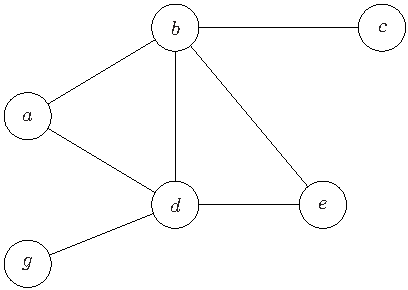
\includegraphics[width=0.5\textwidth]{figs/approxVC-example}      
%     \end{center}

%   \end{itemize}
% \end{frame}
% \begin{frame}
%   \begin{itemize}
%   \item Select edge (randomly) $(b,d)$, add $b$ and $d$ to $C$ then remove $(b,a),(b,c),(b,d),(b,e),(d,a),(d,g)$. Thus $C=\{b,d\}$ and $F=\emptyset$ and the algorithm stops. 
% \item In this case if  we select $(b,d)$ the algorithm gives an exact result and we have $A=\{(b,d)\}$, $C=C^*=\{b,d\}$
% \item What happens if we start from a different edge? say $(b,c)$
% \item $C=\{b,c\}$, $F=\{(a,d),(d,g),(d,e)$.
% \item select (randomly) $(d,g)$
% \item $C=\{b,c,d,g\}$ and $F=\emptyset$ the algorithm stops. In this case size of $VC$ is bigger(by one) than the optimal VC $\{b,d\}$.
% \item Clearly the result depends on our choice of edges.
% \item What is the worst (with respect to the exact result) case of our algorithm? Is there a bound to its difference from the exact result?
% \end{itemize}
% \end{frame}
% \begin{frame}
%   \frametitle{Analysis}
%   \begin{itemize}
%   \item Let $A$ be the set of edges selected in the algorithm on line 4 and Let $C^*$ be the minimal vertex cover.
%   \item two edges in $A$ cannot have a common vertex since when an edge $(u,v)$ is selected all edges incident on $u$ and $v$ are removed from $F$ (in line 6)
%   \item Since $C^*$ is a cover then every edge in $A$ has an endpoint in $C^*$ and since no two edges in $A$ share a vertex then 
%     \begin{align*}
%       |C^*|\ge |A|
%     \end{align*}
% \item But $|C|=2|A|$ therefore
%   \begin{align*}
%     |C|\le 2|C^*|
%   \end{align*}
%   \end{itemize}
% \end{frame}

\end{document}


%%% Local Variables:
%%% mode: latex
%%% TeX-master: t
%%% End:
